\section{Antibiotic derivatives}

\subsection{Ciprofloxacin derivative}

%Ciprofloxacin \compound{cmpd:cip} (see \ref{fgr:cip_num}) is second-generation fluoroquinolone antibiotic used to treat both Gram-positive and Gram-negative bacterial infections\cite{Oliphant2002}.
%The structure-activity relationships for ciprofloxacin have been investigated \cite{Renau1996} and positions 2 and 7 were found not to cause loss of activity. It was therefore decided that alkyne tails would be added at these positions giving two derivatives of ciprofloxacin, \compound{cmpd:hexpipcip} and \compound{cmpd:pipciphex} (see \ref{sch:cip_anas}).

\todo{put intro in intro}

%Three derivatives of ciprofloxacin modified at the free piperazine N were synthesised. These contained a six-carbon alkyl chain with a terminal alkyne, a six-carbon acyl chain with a terminal alkyne and a three carbon acyl chain with a terminal alkyne.

\subsubsection{Retrosynthesis of ciprofloxacin derivative \compound{cmpd:hexpipcip}}

The retrosynthesis of ciprofloxacin derivative \compound{cmpd:hexpipcip} is shown in \ref{sch:hexpipcip_retro}.
The derivative has an alkyne tail attached on the free piperazine N; it is more convenient to attach the alkyne chain to piperazine before coupling of the alkyl piperazine \compound{cmpd:hexpip} to the ciprofloxacin core \compound{cmpd:Clcip} as this method is more convergent. This can be achieved by reductive amination of hex-5-ynal \compound{cmpd:hexynal} with 1-boc-piperazine \compound{cmpd:pipboc} followed by deprotection to form the alkyl piperazine \compound{cmpd:hexpip}. This method was found by Renau \textit{et al.} to be "...superior to previous reports which involved alkylation of piperazine with an appropriate alkyl halide." \cite{Renau1996,JPS:JPS2600571210}. 
S$_N$Ar coupling of the piperazine derivative with ciprofloxacin precursor \compound{cmpd:Clcip} leads to the final derivative \compound{cmpd:hexpipcip}.

\begin{scheme}[H]
	\begin{center}
		\schemeref[hexynol]{cmpd:hexynol}
		\schemeref[hexynal]{cmpd:hexynal}
		\schemeref[pipboc]{cmpd:pipboc}
		\schemeref[hexpipboc]{cmpd:hexpipboc}
		\schemeref[hexpip]{cmpd:hexpip}
		\schemeref[Clcip]{cmpd:Clcip}
		\schemeref[hexpipcip]{cmpd:hexpipcip}
		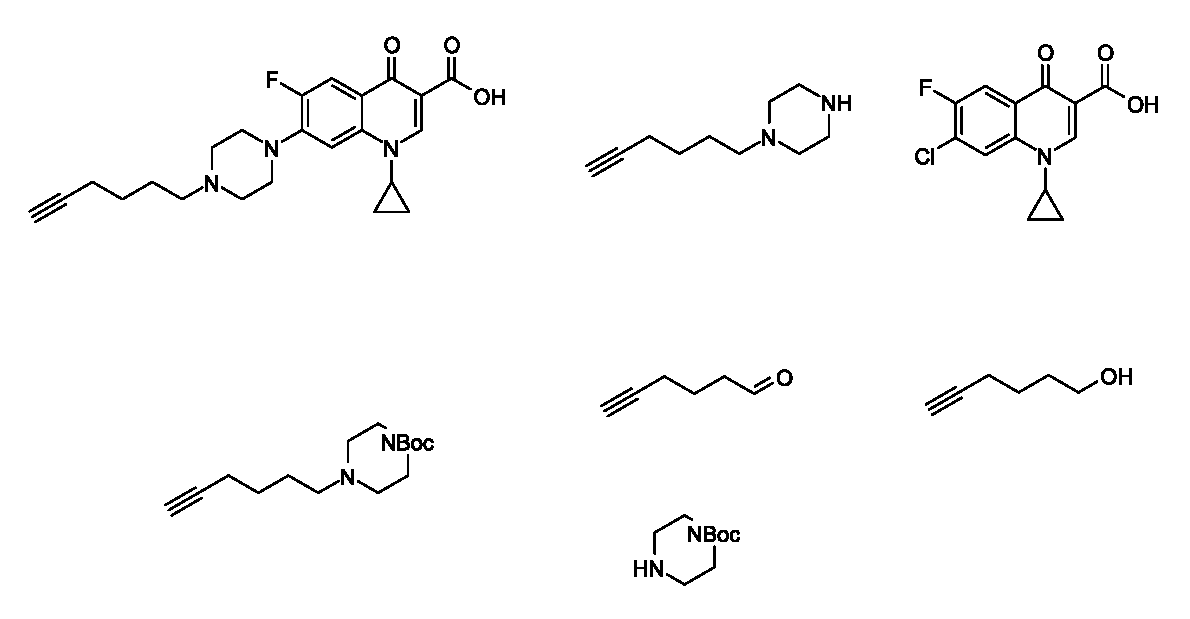
\includegraphics[scale=1]{hexpipcip_retro}
		\caption{The retrosynthesis of \compound{cmpd:hexpipcip}. \label{sch:hexpipcip_retro}}
	\end{center}
\end{scheme}

\subsubsection{Synthesis of ciprofloxacin derivative \compound{cmpd:hexpipcip}}

The synthesis of \compound{cmpd:hexpipcip} follows the strategy followed by Renau \textit{et al.} \cite{Renau1996}. Unlike the aldehydes and ketones used by Renau \textit{et al.}\cite{Renau1996}, hex-5-ynal \compound{cmpd:hexynal} is not commercially available and so was successfully prepared by PCC oxidation of hex-5-ynol \compound{cmpd:hexynol} according to the procedure described by Kocsis \textit{et al.} \cite{Kocsis2012}. Renau \textit{et al.}\cite{Renau1996} used sodium cyanoborohydride to facilitate the reductive amination of hex-5-ynal \compound{cmpd:hexynal} and 1-Boc-piperazine \compound{cmpd:pipboc}. However, it was decided to attempt this transformation using the less toxic sodium triacetoxyborohydride following a procedure reported by Abdel-Magid \textit{et al.} \cite{Abdel-Magid1996}. This reaction yielded compound \compound{cmpd:hexpipboc}, which was deprotected using TFA using the procedure described by Renau \textit{et al.}\cite{Renau1996} to give compound \compound{cmpd:hexpip}. This was refluxed in MeCN with the commercially available ciprofloxacin precursor \compound{cmpd:Clcip} according to the procedure described by Renau \textit{et al.}\cite{Renau1996}, however the reaction did not proceed. Addition of \ce{NEt3} did not lead to reaction, however it was found that refluxing in neat \ce{NEt3} lead to conversion to the final ciprofloxacin derivative \compound{cmpd:hexpipcip}.

\begin{scheme}[H]
	\begin{center}
		\schemeref[hexynol]{cmpd:hexynol}
		\schemeref[hexynal]{cmpd:hexynal}
		\schemeref[pipboc]{cmpd:pipboc}
		\schemeref[hexpipboc]{cmpd:hexpipboc}
		\schemeref[hexpip]{cmpd:hexpip}
		\schemeref[Clcip]{cmpd:Clcip}
		\schemeref[hexpipcip]{cmpd:hexpipcip}
		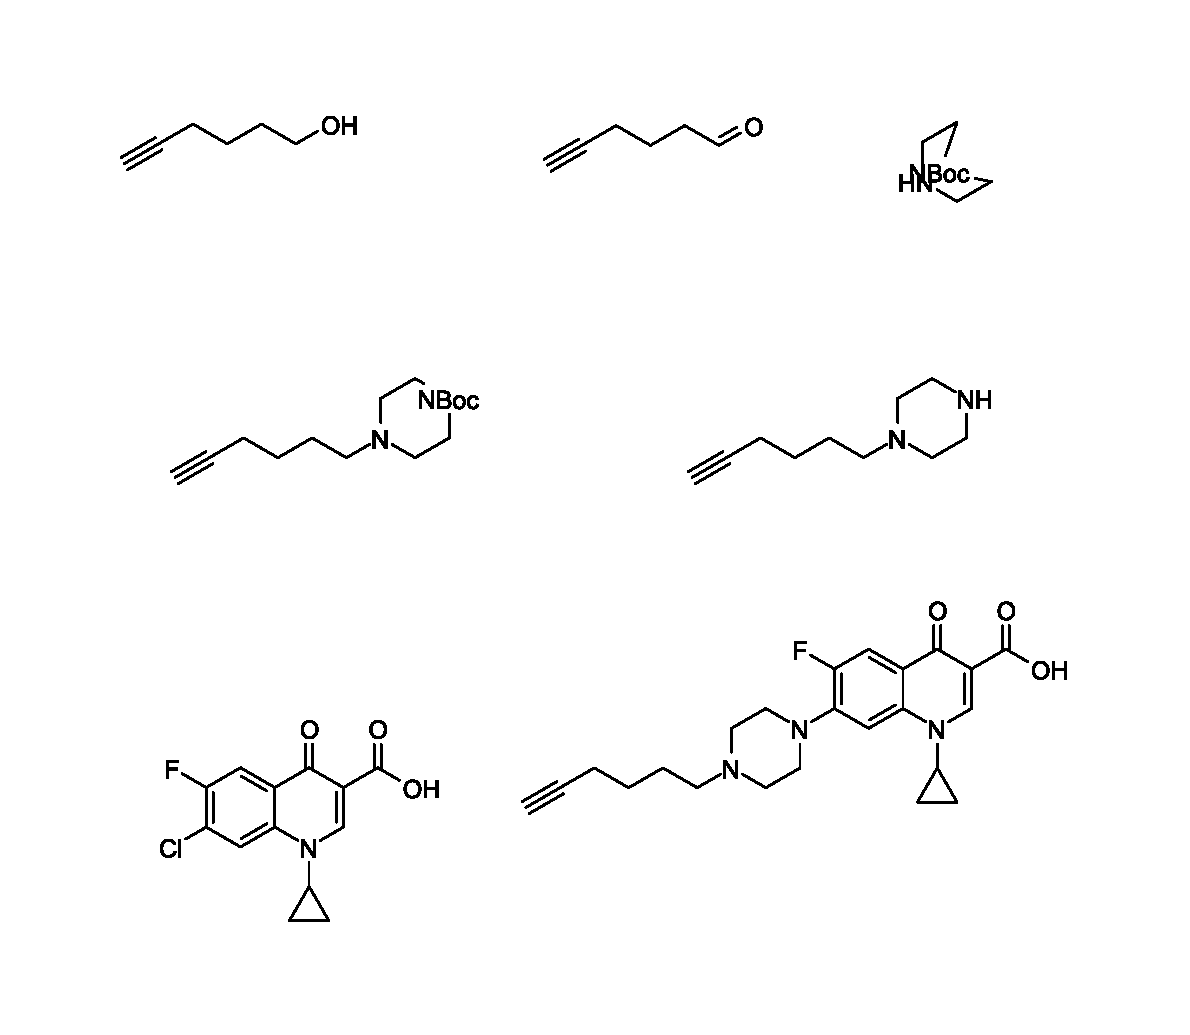
\includegraphics[scale=1]{hexpipcip_synth}
		\caption{The synthesis of \compound{cmpd:hexpipcip}. 
		a) Pyridinium chlorochromate, \ce{CH2Cl2}, r.t., 5 h, 72 \%.
		b) \ce{NaBH(AcO)3}, 1,2-dichloroethane, r.t., 10.5 h, 99 \%.
		c) TFA, r.t., 1 h, 100 \%.
		d) \ce{NEt3}, reflux, 15 h, 21 \%. %weigh
		\label{sch:hexpipcip_synth}}
	\end{center}
\end{scheme}

\subsection{Trimethoprim derivative}

\begin{scheme}[H]
	\begin{center}
		\schemeref[Tri]{cmpd:Tri}
		\schemeref[TriOH]{cmpd:TriOH}
		\schemeref[Cl4Y]{cmpd:Cl4Y}
		\schemeref[Y4Tri]{cmpd:Y4Tri}
		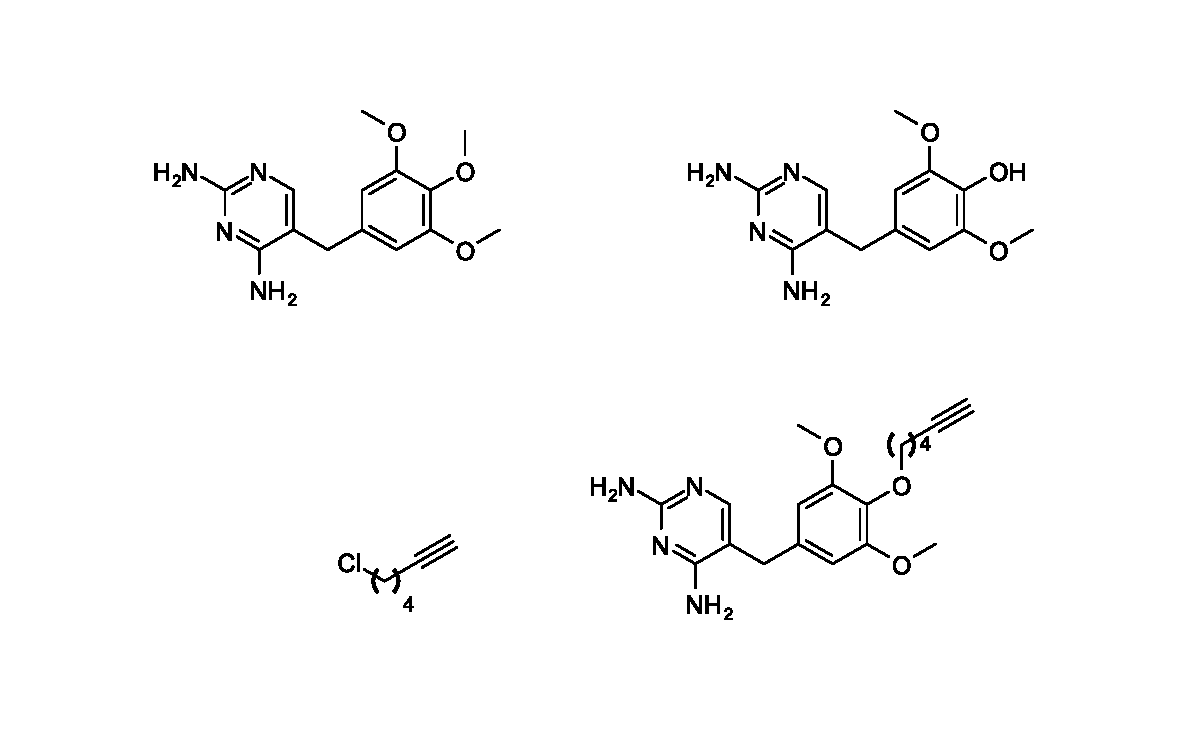
\includegraphics[scale=1]{Y4Tri_synth}
		\caption{The synthesis of \compound{cmpd:Y4Tri}.\label{sch:Y4Tri_synth}}
	\end{center}
\end{scheme}

\todo{discuss this}